\section{Codierung}

\subsection{Lauflängen-Codierung}

Die Lauflängenkodierung komprimiert verlustfrei längere Abfolgen gleicher Symbole.

\begin{lstlisting}
AAAAA => 5A
\end{lstlisting}

Sind bei einem Bild z. B. 100 Pixel, die aufeinander Folgen, weiß,
so muss nur noch 1 Pixel und die Anzahl gespeichert werden. Wenn 1 Pixel
24 Bit groß ist, werden so unfähr 2,4 Kilobyte eingespart.

\subsection{Huffman-Codierung}

Bei der Huffman Codierung wird die Gesamtlänge der Daten dadurch reduziert,
dass häufig vorkommende Symbole mit kürzeren Bitfolgen kodiert werden und
selten vorkommende Symbole mit längeren Bitfolgen. Dadurch lässt sich die Gesamtlänge
meist deutlich reduzieren. Je größer die Entropie der zu Kodierenden Symbole, desto
höher ist die Kompressionsrate.

Die resultierende Kodierung für eine Menge an Symbolen ist ein Präfixcode
(erfüllt Fano-Bedingung).
Das heißt, dass keine Bitfolge zur kodierung eines Symbols zu Beginn einer
anderen Bitfolge zu finden ist. Somit ist es immer klar möglich, die Bitfolge
einem Symbol zuzuordnen und festzustellen, wann die Bitfolge zuende ist.
Um die Huffmann-Kodierung praktisch zu nutzen, muss die Huffmann-Kodierung
zur decodierung allerdings immer mitgeliefert werden und verbraucht auch Platz.
Lohnenswert ist die Huffmann-Kodierung also nur, wenn die Einsparungen größer sind als
der Platz, den die Dekodierungstabelle verbraucht. 

\subsubsection{Erstellung einer Huffman-Kodierung}

Beim ASCII Code wird jedes Zeichen mit 8 Bit kodiert.
Für jeden bestimmten Text lässt sich allerdings eine auf diesen
zugeschnitte, meist bessere, Huffmann-Kodierung generieren.
Zuerst werden die Häufigkeiten der Zeichen bestimmt.

\begin{lstlisting}
ABACEADBCEEEC
A: 3
B: 2
C: 3
D: 1
E: 4
Gesamt: 13
\end{lstlisting}

\clearpage

Anschließend lässt sich die individuelle Kodierung über einen Huffmann-Baum erstellen.
Es werden alle Häufigkeiten als Knoten betrachtet. Dann wird folgendes solange
wiederholt, bis es nur noch 1 Baum gibt. Dabei können für gleiche Symbolfolgen auch
mehrere unterschiedliche, aber alle valide, Bäume entstehen.

\begin{enumerate}
    \item Wähle die Teilbäume mit der geringsten absoluten/relativen Häufigkeit in
    der Wurzel. Bei gleicher Häufigkeit wähle den Teilbaum mit der geringeren Tiefe.
    \item Fasse diese zu einem neuen Teilbaum zusammen, in dessen Wurzel die Summe
    der Häufigkeiten der Wurzeln der Teilbäume steht.
    (Teilbaum mit geringerer Häufigkeit möglichst immer auf der gleichen Seite für optimale Kodierung)
\end{enumerate}

\vspace*{0.5cm}

\begin{forest}
for tree={
    grow=south,
    circle, draw, minimum size=5ex, inner sep=3pt,
    s sep=7mm
}
[, phantom, s sep = 7mm
    [A: 3]
    [B: 2]
    [C: 3]
    [D: 1]
    [E: 4]
]
\end{forest}

\vspace*{1cm}

\begin{forest}
for tree={
    grow=south,
    circle, draw, minimum size=5ex, inner sep=3pt,
    s sep=7mm
}
[, phantom, s sep = 7mm
    [3
        [D: 1]
        [B: 2]
    ]
    [3, phantom, s sep = 7mm
        [A: 3]
        [C: 3]
        [E: 4]
    ]
]
\end{forest}

\vspace*{1cm}

\begin{forest}
for tree={
    grow=south,
    circle, draw, minimum size=5ex, inner sep=3pt,
    s sep=7mm
}
[, phantom, s sep = 7mm
    [3
        [D: 1]
        [B: 2]
    ]
    [6
        [A: 3]
        [C: 3]
    ]
    [, phantom, s sep = 7mm
        [E: 4]
    ]
]
\end{forest}

\vspace*{1cm}

\begin{forest}
for tree={
    grow=south,
    circle, draw, minimum size=5ex, inner sep=3pt,
    s sep=7mm
}
[, phantom, s sep = 7mm
    [7
        [3
            [D: 1]
            [B: 2]
        ]
        [E: 4]
    ]
    [6
        [A: 3]
        [C: 3]
    ]
]
\end{forest}

\begin{forest}
for tree={
    grow=south,
    circle, draw, minimum size=5ex, inner sep=3pt,
    s sep=7mm
}
[13
    [6
        [A: 3]
        [C: 3]
    ]
    [7
        [3
            [D: 1]
            [B: 2]
        ]
        [E: 4]
    ]
]
\end{forest}

\vspace*{0.5cm}

Nun werden Nullen und Einsen an den Kanten eingetragen und für jedes Symbol
lässt sich die Kodierung anhand der Zahlen am Pfad von der Wurzel ausgehend
bestimmten. Die Buchstaben D und B kommen am seltensten vor. Man erkennt,
dass diese mit der längsten Bitsequenz kodiert werden. Häufiger vorkommende
Buchstaben werden kürzer kodiert. Die mit Huffmann kodierte Nachricht ist auch klar
kürzer, doch muss immer die Dekodierungstabelle mitgeliefert werden.

\vspace*{0.5cm}

\begin{forest}
for tree={
    grow=south,
    circle, draw, minimum size=5ex, inner sep=3pt,
    s sep=7mm,
    EL/.style = {edge label={node[midway, fill=white, inner sep=2pt, anchor=center]{#1}},},
}
[13
    [6, EL=0
        [A: 3, EL=0]
        [C: 3, EL=1]
    ]
    [7, EL=1
        [3, EL=0
            [D: 1, EL=0]
            [B: 2, EL=1]
        ]
        [E: 4, EL=1]
    ]
]
\end{forest}

\vspace*{0.5cm}

\begin{lstlisting}
A: 00
B: 101
C: 01
D: 100
E: 11
ABACEADBCEEEC =ASCII=> 
01000001 01000010 01000001 01000011 01000101 01000001 01000100 01000010
01000011 01000101 01000101 01000101 01000011
ABACEADBCEEEC =HUFF==>
00 101 00 01 11 00 100 101 01 11 11 11 01
\end{lstlisting}

\subsection{Deflate Kompression}

Der z. B. bei Zip-Dateien genutzte Kompressionsalgorithmus Deflate kombiniert
die Huffmann-Kodierung mit einer LZ-Variation. Dadurch können Daten verlustfrei
komprimiert werden, indem der von häufig vorkommenden und von sich wiederholenden
Daten eingenomme Platz reduziert wird. 

\subsection{Hamming Code}

Der Hamming Code ist ein Fehlerkorrekturcode um 1 Bit Fehler in Bitfolgen
zu erkennen und zu korrigieren. Dabei zeichnet sich dieser dadurch aus,
dass nur wenige Paritätsbits benötigt werden, auch bei großen Bitfolgen.

Der Hamming Code funktioniert so, dass zu den 4 Datenbits 3 Paritätsbits
hinzugefügt werden (gesamt 7 Bits). Die Paritätsbits werden so gesetzt,
dass die Summe in alle Kreisen gerade (oder ungerade) ist. Es ist nur wichtig,
dass bei der Prüfung dies bekannt ist.

\begin{table}[H]
    \begin{tabular}{|l|l|l|}
    \hline
        Bit & Ursprungs Nachricht & Fehlerhafte Nachricht \\ \hline
        $d_1$ & 1 & 1 \\ \hline
        $d_2$ & 0 & 0 \\ \hline
        $d_3$ & 0 & 1 \\ \hline
        $d_4$ & 1 & 1 \\ \hline
        $p_1$ & 0 & 0 \\ \hline
        $p_2$ & 0 & 0 \\ \hline
        $p_3$ & 1 & 1 \\ \hline
    \end{tabular}
\end{table}

Summiert man jeweils die Kreis so erhält man für die Ursprungsnachricht
jeweils korrekte, gerade Ergebnisse. Bei der Fehlerhaften Nachricht (z. B. durch
Übertragungsfehler), wo ein Bit getauscht wurde, erhält man hingegen unpassende,
ungerade Ergebnisse.

\begin{align*}
red_u & = d_2 + d_3 + d_4 + p_3 = 0 + 0 + 1 + 1 = 2 \\
green_u & = d_1 + d_2 + d_4 + p_1 = 1 + 0 + 1 + 0 = 2 \\
blue_u & = d_1 + d_3 + d_4 + p_2 = 1 + 0 + 1 + 0 = 2 \\
& \\
red_f & = d_2 + d_3 + d_4 + p_3 = 0 + 1 + 1 + 1 = 3 \\
green_f & = d_1 + d_2 + d_4 + p_1 = 1 + 0 + 1 + 0 = 2 \\
blue_f & = d_1 + d_3 + d_4 + p_2 = 1 + 1 + 1 + 0 = 3 \\
\end{align*}

\vspace*{-1cm}

\begin{figure}[H]
    \centering
    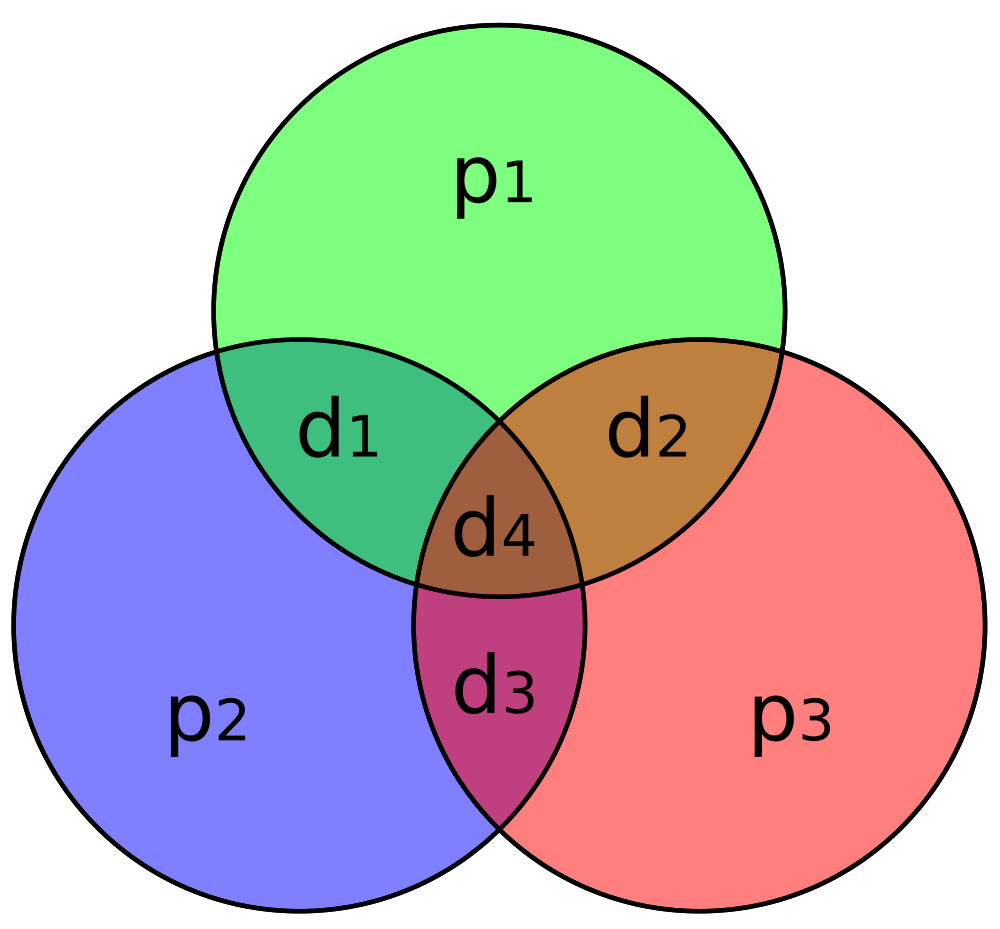
\includegraphics[width=0.5\textwidth]{images/hamming7.4.png}
    \caption{\textbf{7,4 Hamming Code}}
\end{figure}

Wenn man davon ausgeht, das 1 Bit getauscht wurde, so lässt sich erkennen,
das nur in den Kreisen Rot und Blau die Summe nicht passt. Das Bit kann
sich also nicht im Grünen Kreis befinden. Die einzige Überschneidung
von Rot und Blau ist $d_3$, weswegen sich das getauschte Bit dort befinden
muss. Dieses kann nun zurückgetauscht werden, wodurch die ursprüngliche Nachricht
wiederhergestellt wird. Sind allerdings 2 oder mehr Bits getauscht, so kann dies
nicht erkannt werden. Der 8,4 Hamming Code ermöglicht es allerdings zu erkennen, wenn
2 Bits getauscht sind, aber nicht diese auch zu korrigieren.

\begin{figure}[H]
    \centering
    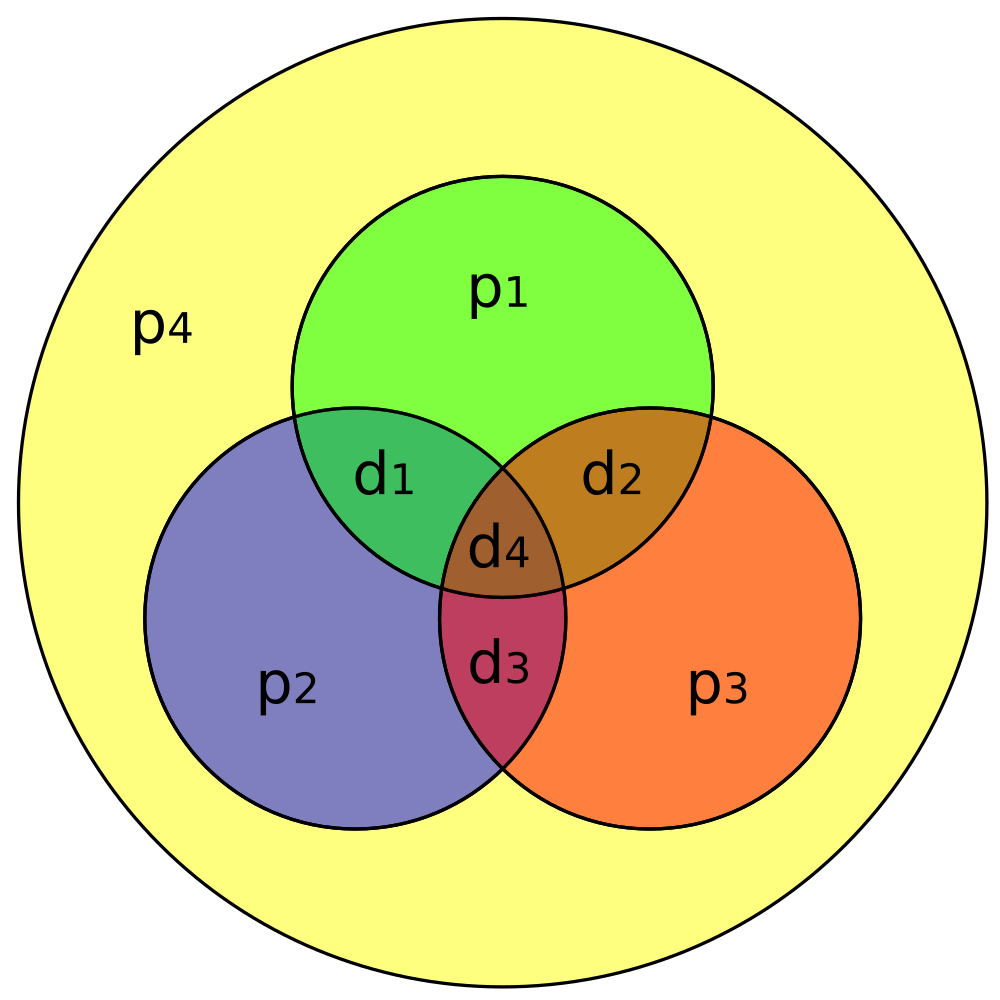
\includegraphics[width=0.4\textwidth]{images/hamming8.4.png}
    \caption{\textbf{8,4 Hamming Code}}
\end{figure}

\href{https://www.youtube.com/watch?v=X8jsijhllIA}{3B1B Hamming Codes Video}

\subsection{Bildkodierung}

Bei einem Bild wird die Farbe eines Pixel Grundsätzlich durch 3 Werte, einen Rot,
Grün und Blau Wert festgelegt und so gespeichert. Diese Werte können dabei jeweils
8, 10, 16 oder mehr Bit groß sein, wodurch sich der Farbraum der Pixel vergrößert.
Zusätzlich kann noch die Transparenz eines Pixels gespeichert werden, der Alpha Wert.
Je nach Bitanzahl pro Pixel und Kompression unterscheiden sich so Bilder verschiedener
Qualitäten und Formate (e.g. JPG, PNG). Meist werden Bilder mit 8 Bit Werten gespeichert,
also 8 Bit jeweils für Rot, Grün, Blau. Jede Farbe hat somit einen Wert zwischen 0 und 255.
Ein Pixel kann also $255^3$ unterschiedliche Farben annehmen. Das sind ca. 16,7 Millionen
Farben.

\begin{figure}[H]
    \centering
    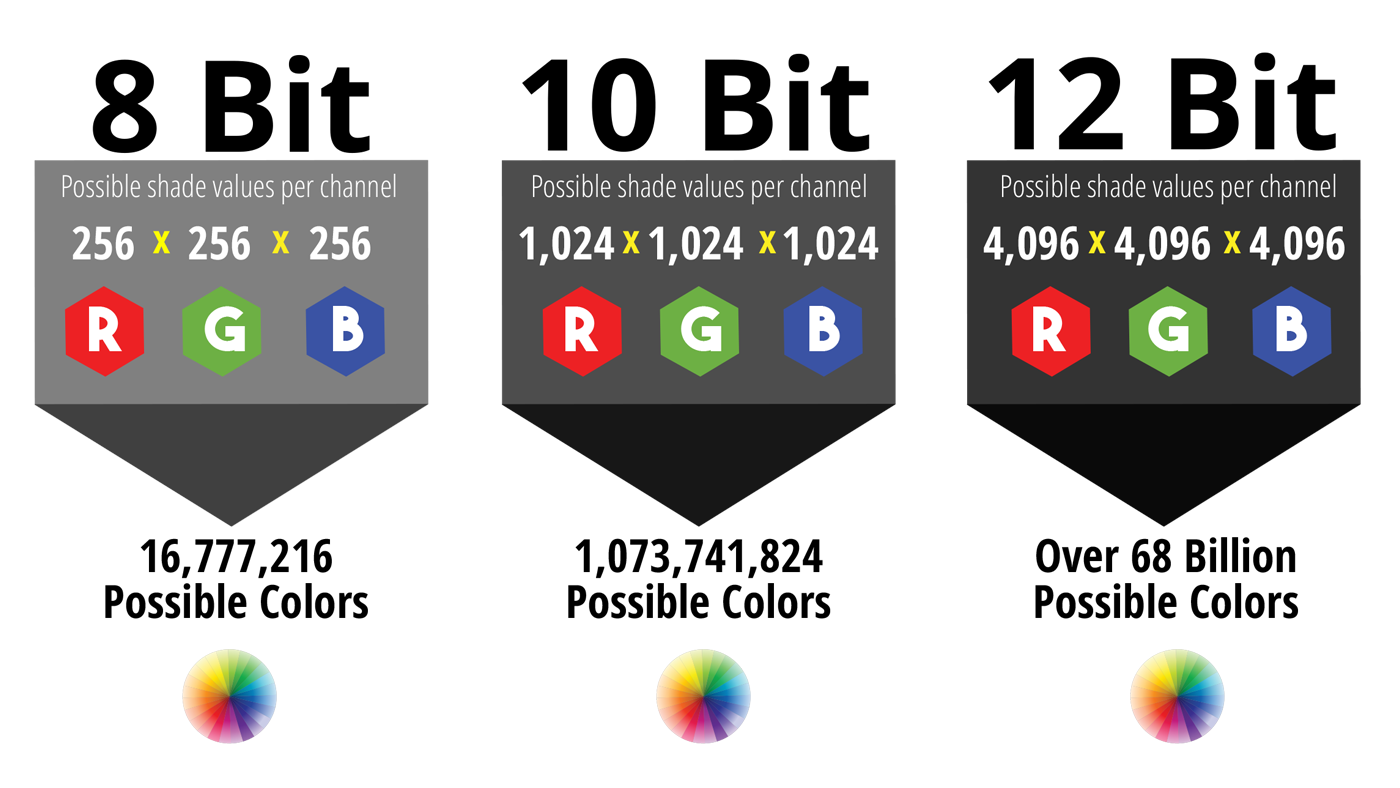
\includegraphics[width=0.8\textwidth]{images/rgbvalues.png}
    \caption{\textbf{Verschiedene Farbtiefen bei Bildern}}
\end{figure}
